\documentclass[11pt, letterpaper, twoside]{article}
\usepackage[utf8]{inputenc}
\usepackage[symbol]{footmisc}
\usepackage{hyperref}
\usepackage{amsmath}
\usepackage{amssymb}
\usepackage{listings}
\usepackage{algpseudocode}
\usepackage{algorithm}
\usepackage{graphicx}
\usepackage{multirow}
\usepackage{subcaption}
\usepackage{bigfoot} % for verbatim in footnotes

\graphicspath{{./plots/}}
\renewcommand{\figurename}{Benchmark}
 
\renewcommand{\thefootnote}{\fnsymbol{footnote}}
% usage \footnote[num]{text}
% with num in [1..9]
% 1   asterisk    *   2   dagger  †   3   double dagger   ‡
% 4   section symbol  §   5   paragraph   ¶   6   parallel lines  \\
% 7   two asterisks   **  8   two daggers ††  9   two double daggers  ‡‡

\textwidth=16cm 
\oddsidemargin=0cm
\evensidemargin=0cm

\begin{document}

\title{Benchmark Results for Gap Decorator Variants}
\maketitle 

\section{The Approaches}
Three gap decorator variations were benchmarked against each other and against a sequence allowing regular \verb|seqan3::dna15| letters and the \verb|gap::GAP| symbol. Let's denote with $n$ the ungapped sequence length, $k$ the number of gaps (not number of gap symbols!) and $m$ the number of gap symbols. 
\begin{enumerate}
    \item {\bf Gapped Sequence} An \verb|std::vector| of type \verb|gapped<dna15>| which grows and shrinks on direct insertion/deletion of gaps.
	\begin{itemize}
		\item Direct addressing
		\item Overhead because of explicit gap character storage
		\item \verb|dna| cast to wider data type \verb|gapped<dna>|
	\end{itemize}
    \item {\bf Gap vector} Using a compressed bit vector of length $|$sequence$|$ + \# gaps
    \begin{itemize}
        \item Bit vector is \verb|sdsl::sd_vector| with rank and select support structures with access time depending on the number of bits set.
        \item Set bit indicates gap, else underlying sequence minus the rank
        \item Bit vectors are not modifyable (except the \verb|sdsl::int_vector|), hence any insertion or deletion operation results in a rebuilt with costs of $\Theta(n)$
    \end{itemize}
    \item {\bf Anchor List} Gaps are stored as anchors, i.e. a list of tuples with {\bf container-relative} positions and lengths of gaps
    \begin{itemize}
        \item Insertion, deletion, and random access positions are virtual (=gapped sequence space), the anchor gaps have to be therefore accumulated to compute the virtual position
    \end{itemize}
    \item {\bf Anchor set} A red-black tree stores the {\bf virtual} anchor positions, an additional dictionary resolves the gap length for a given position.
	\begin{itemize}
		\item An \verb|std::set|\footnote{which is implemented via a red-black tree} is used for key management. The \verb|std::set| does not allow handing over a lambda function for user-defined sorting. Therefore, key-value tuples which have to be sorted only by key cannot be used when one needs the guarantee of $\log_2(k)$ access time.   
		\item Associated gap lengths are stored in an \verb|std::unordered_map| with constant access, but larger storage consumption.
		\item To improve random access runtimes from $\Theta(k)$ to $\Theta(\log_2 k)$, the gap lengths are stored in an accumulated fashion. To retrieve the actual gap length one substracts the accumulator of the preceeding gap.
	\end{itemize}
\end{enumerate}

\begin{table}[htpb]\centering
%\small{
\begin{tabular}{|l|l|l|l|l|}
\hline
\bf Operation&\bf Gapped Sequence&\bf Gap Vector&\bf Anchor List&\bf Anchor Set\\
\hline
\verb|operator[]|&$\Theta(1)$&$\mathcal{O}(\log(\frac{n+m}{m}))$\footnotemark&$\Theta(k)$&$\Theta(\log_2 k)$\\
\verb|erase_gap|&$\Theta(n+m)$&$\Theta(n+m)$&$\Theta(k)$&$\Theta(\log_2 k)$\\
\verb|insert_gap|&$\Theta(n+m)$&$\Theta (n+m)$&$\Theta(k)$&$\Theta(\log_2 k)$\\
\hline
\end{tabular}\caption{Theoretical runtimes and space consumptions with $k$ = number of gaps, $m$ = accumulated gap length, $n$ = underlying (gap-free) sequence length.}	
%} % small
\end{table}
\footnotetext{i.e. costs of \verb|rank_support_sd|}

\begin{table}[htpb]\centering
{\small
\begin{tabular}{|l|l|l|l|l|l|}
\hline
\multicolumn{2}{|c}{}&\bf Gapped Sequence&\bf Gap Vector&\bf Anchor List&\bf Anchor Set\\
\hline
\multicolumn{2}{|l}{Theoretical Space}&$\Theta \big ( (n+m)\cdot |$\verb|gapped<dna>|$|\big )$&$\Theta \big ( m(2+\log \frac{n}{m}) + n\cdot|$\verb|dna|$|\big ) $&$\Theta (k + n\cdot |$\verb|dna|$|)$&$\Theta (k+ n\cdot |$\verb|dna|$|)$\\
\hline
\multirow{2}{*}{Actual Space}&\verb|dna15|&&&&\\
&\verb|dna4|&&&&\\ 
\hline
\end{tabular}\caption{Theoretical and actual space consumptions with $k$ = number of gaps, $m$ = accumulated gap length, $n$ = underlying (gap-free) sequence length including the unaligned sequence. The actual space consumption was measured with valgrind's massif.}	
}
\end{table}


\section{Benchmark Results}
To create realistic gapped sequences or gaps for insertion, gap lengths are sampled from a histogram distribution published by Goonesekere et al. \footnote{see Table 1 in \url{https://www.ncbi.nlm.nih.gov/pmc/articles/PMC419611/}, columns were summed up and normalized} for each position, which results in a rather dense distribution of short gaps (40\%-45\% gap proportion). After sampling, the \lq\lq gapped\rq\rq{} sequences were resized to have total sequence size of $2^i$. All four data structures are then initialized with the same gap vector within the same experiment. Each experiment is repeated 32 times for sequences with lengths in range $[2, 2^2, ..., 2^{15}]$, and 8 times for lengths in range $[2^{16}, ...,2^{18}]$. The benchmarks cover three user scenarios:
\begin{description}
    \item[Benchmark 1] Read-only on ungapped or gapped sequence
    \item[Benchmark 2] Insert/Delete at {\bf random positions} into ungapped or gapped sequence
    \item[Benchmark 3] Insert/Delete from {\bf left to right} into ungapped or gapped sequence
\end{description}

\begin{figure}[htpb]\centering
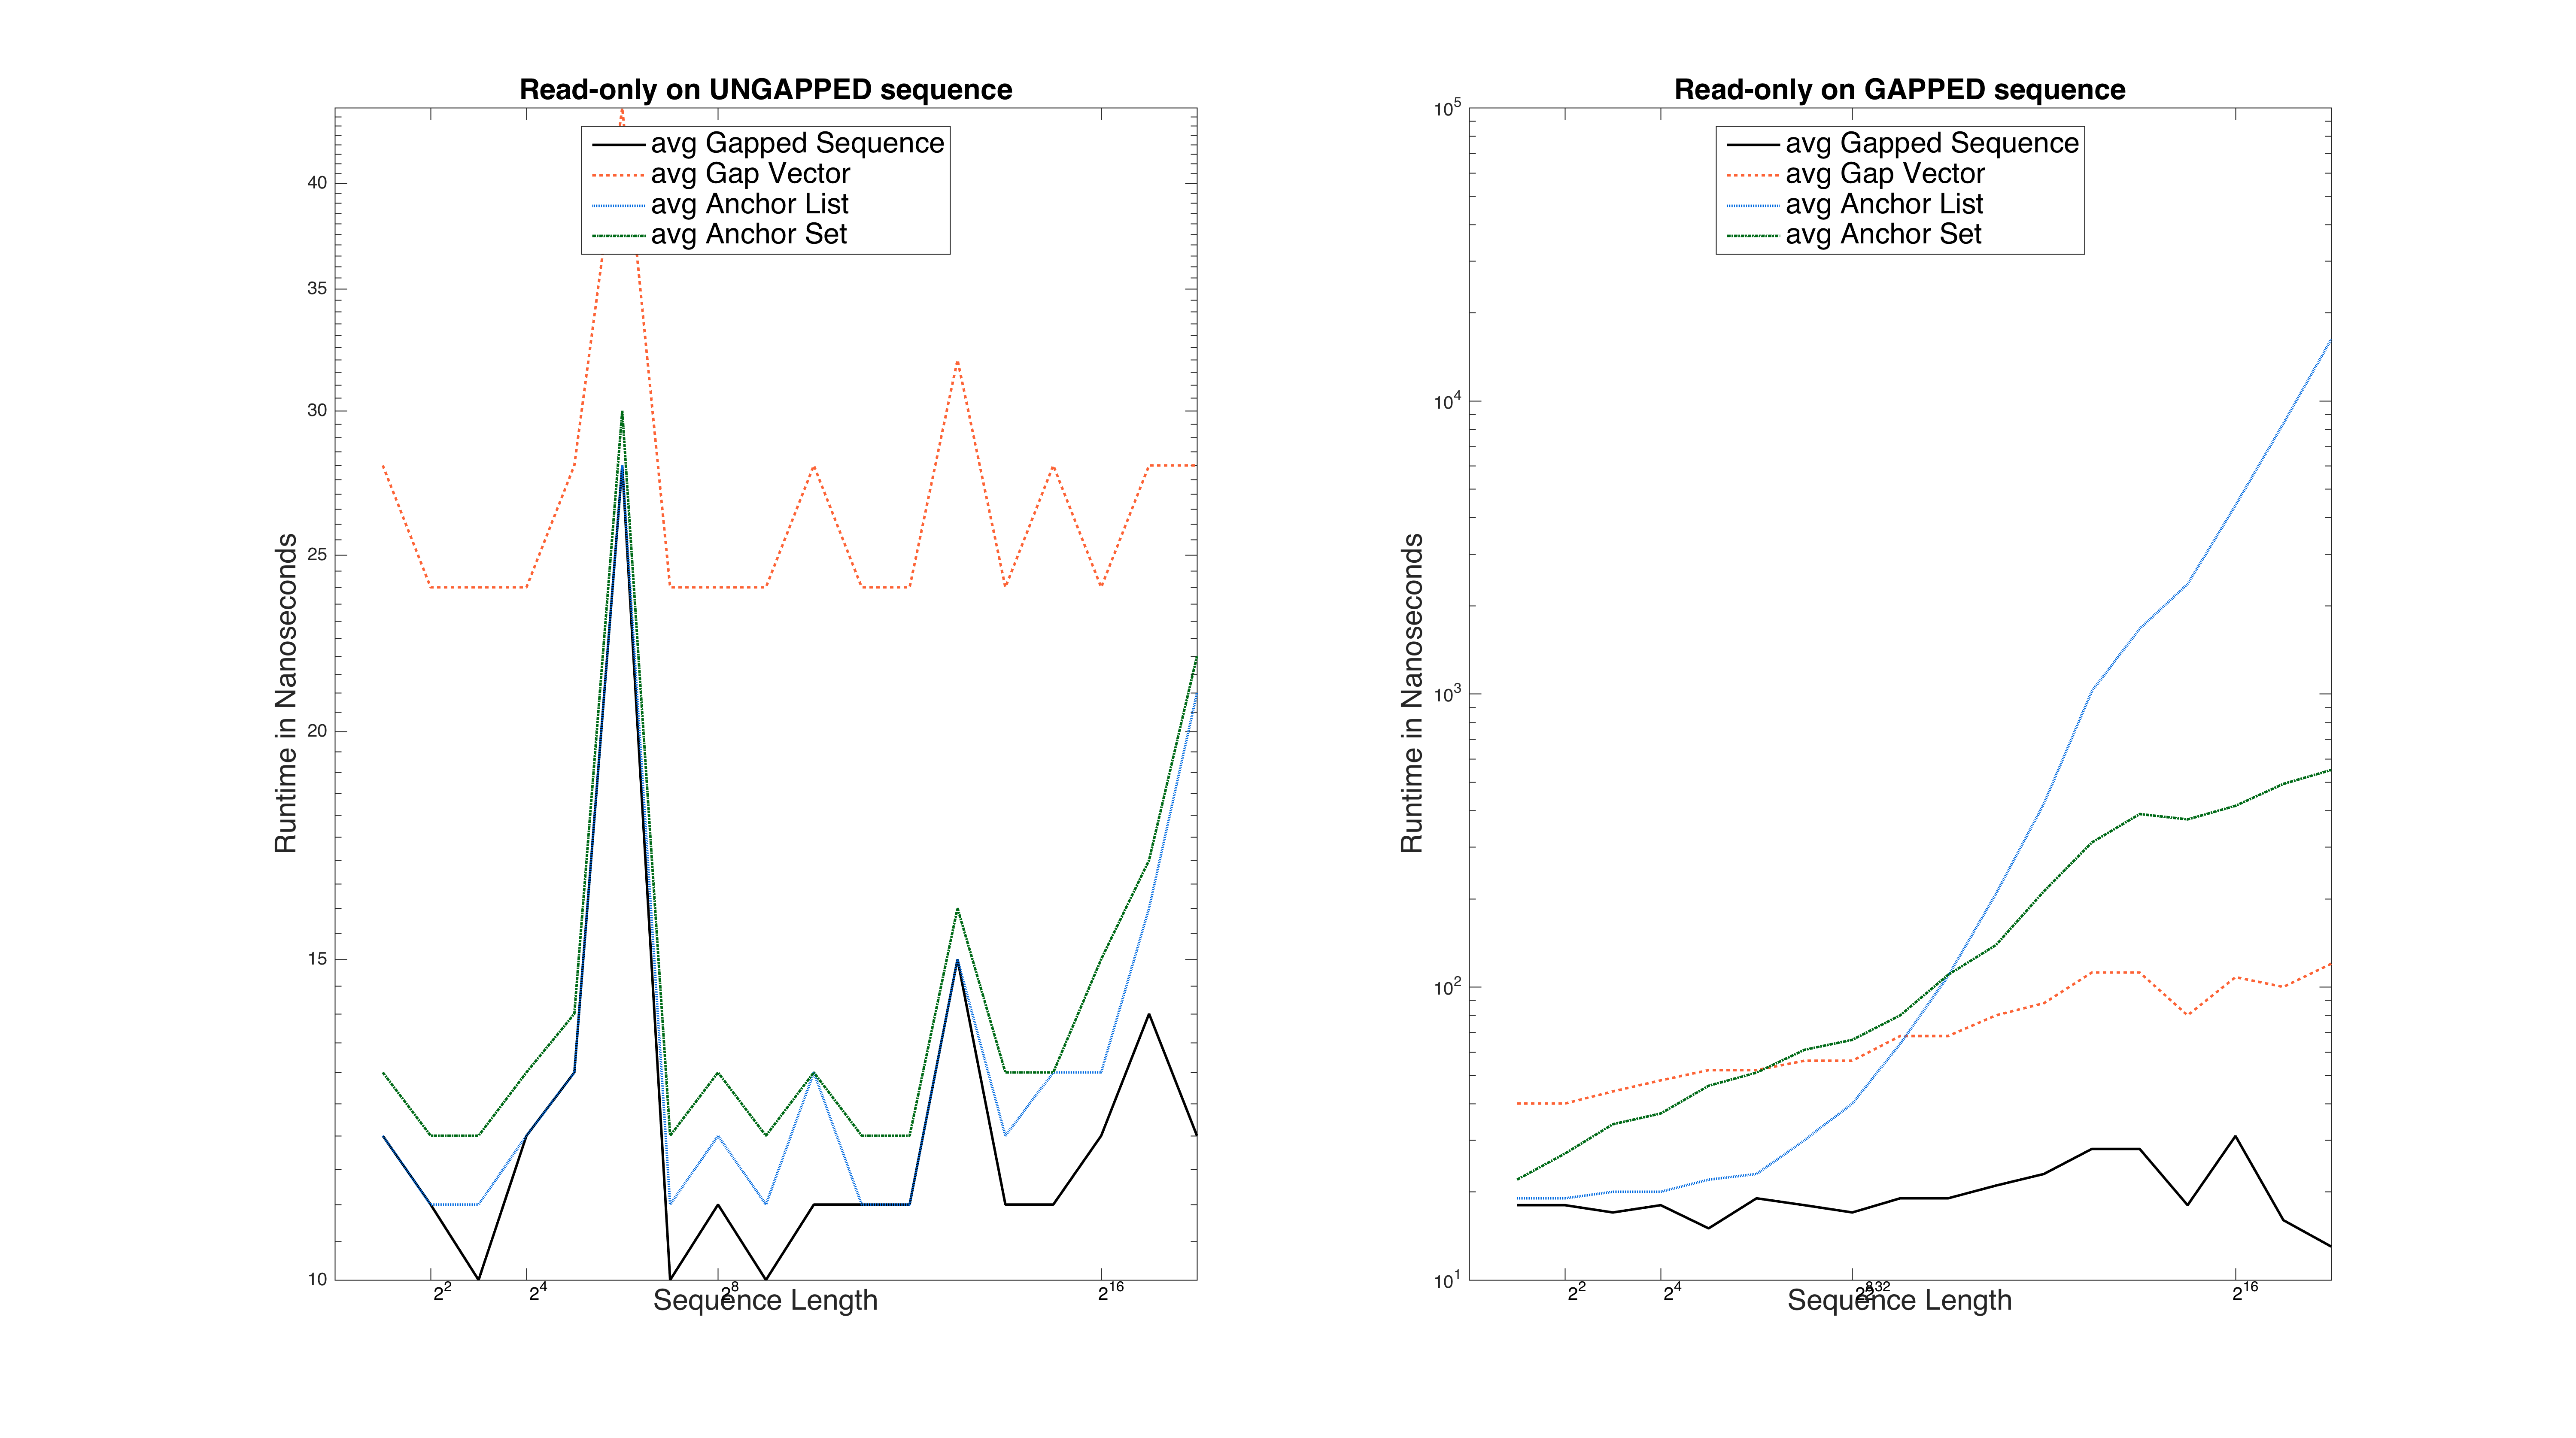
\includegraphics[scale=.4,trim={5cm 2cm 4.5cm 1.5cm},clip]{benchmark1_plot.png}
\caption{Left: Read-only on ungapped sequence, i.e. gap structures are empty. Right: 
Read-only on gapped sequence.}
\end{figure}

\begin{figure}[htpb]\centering
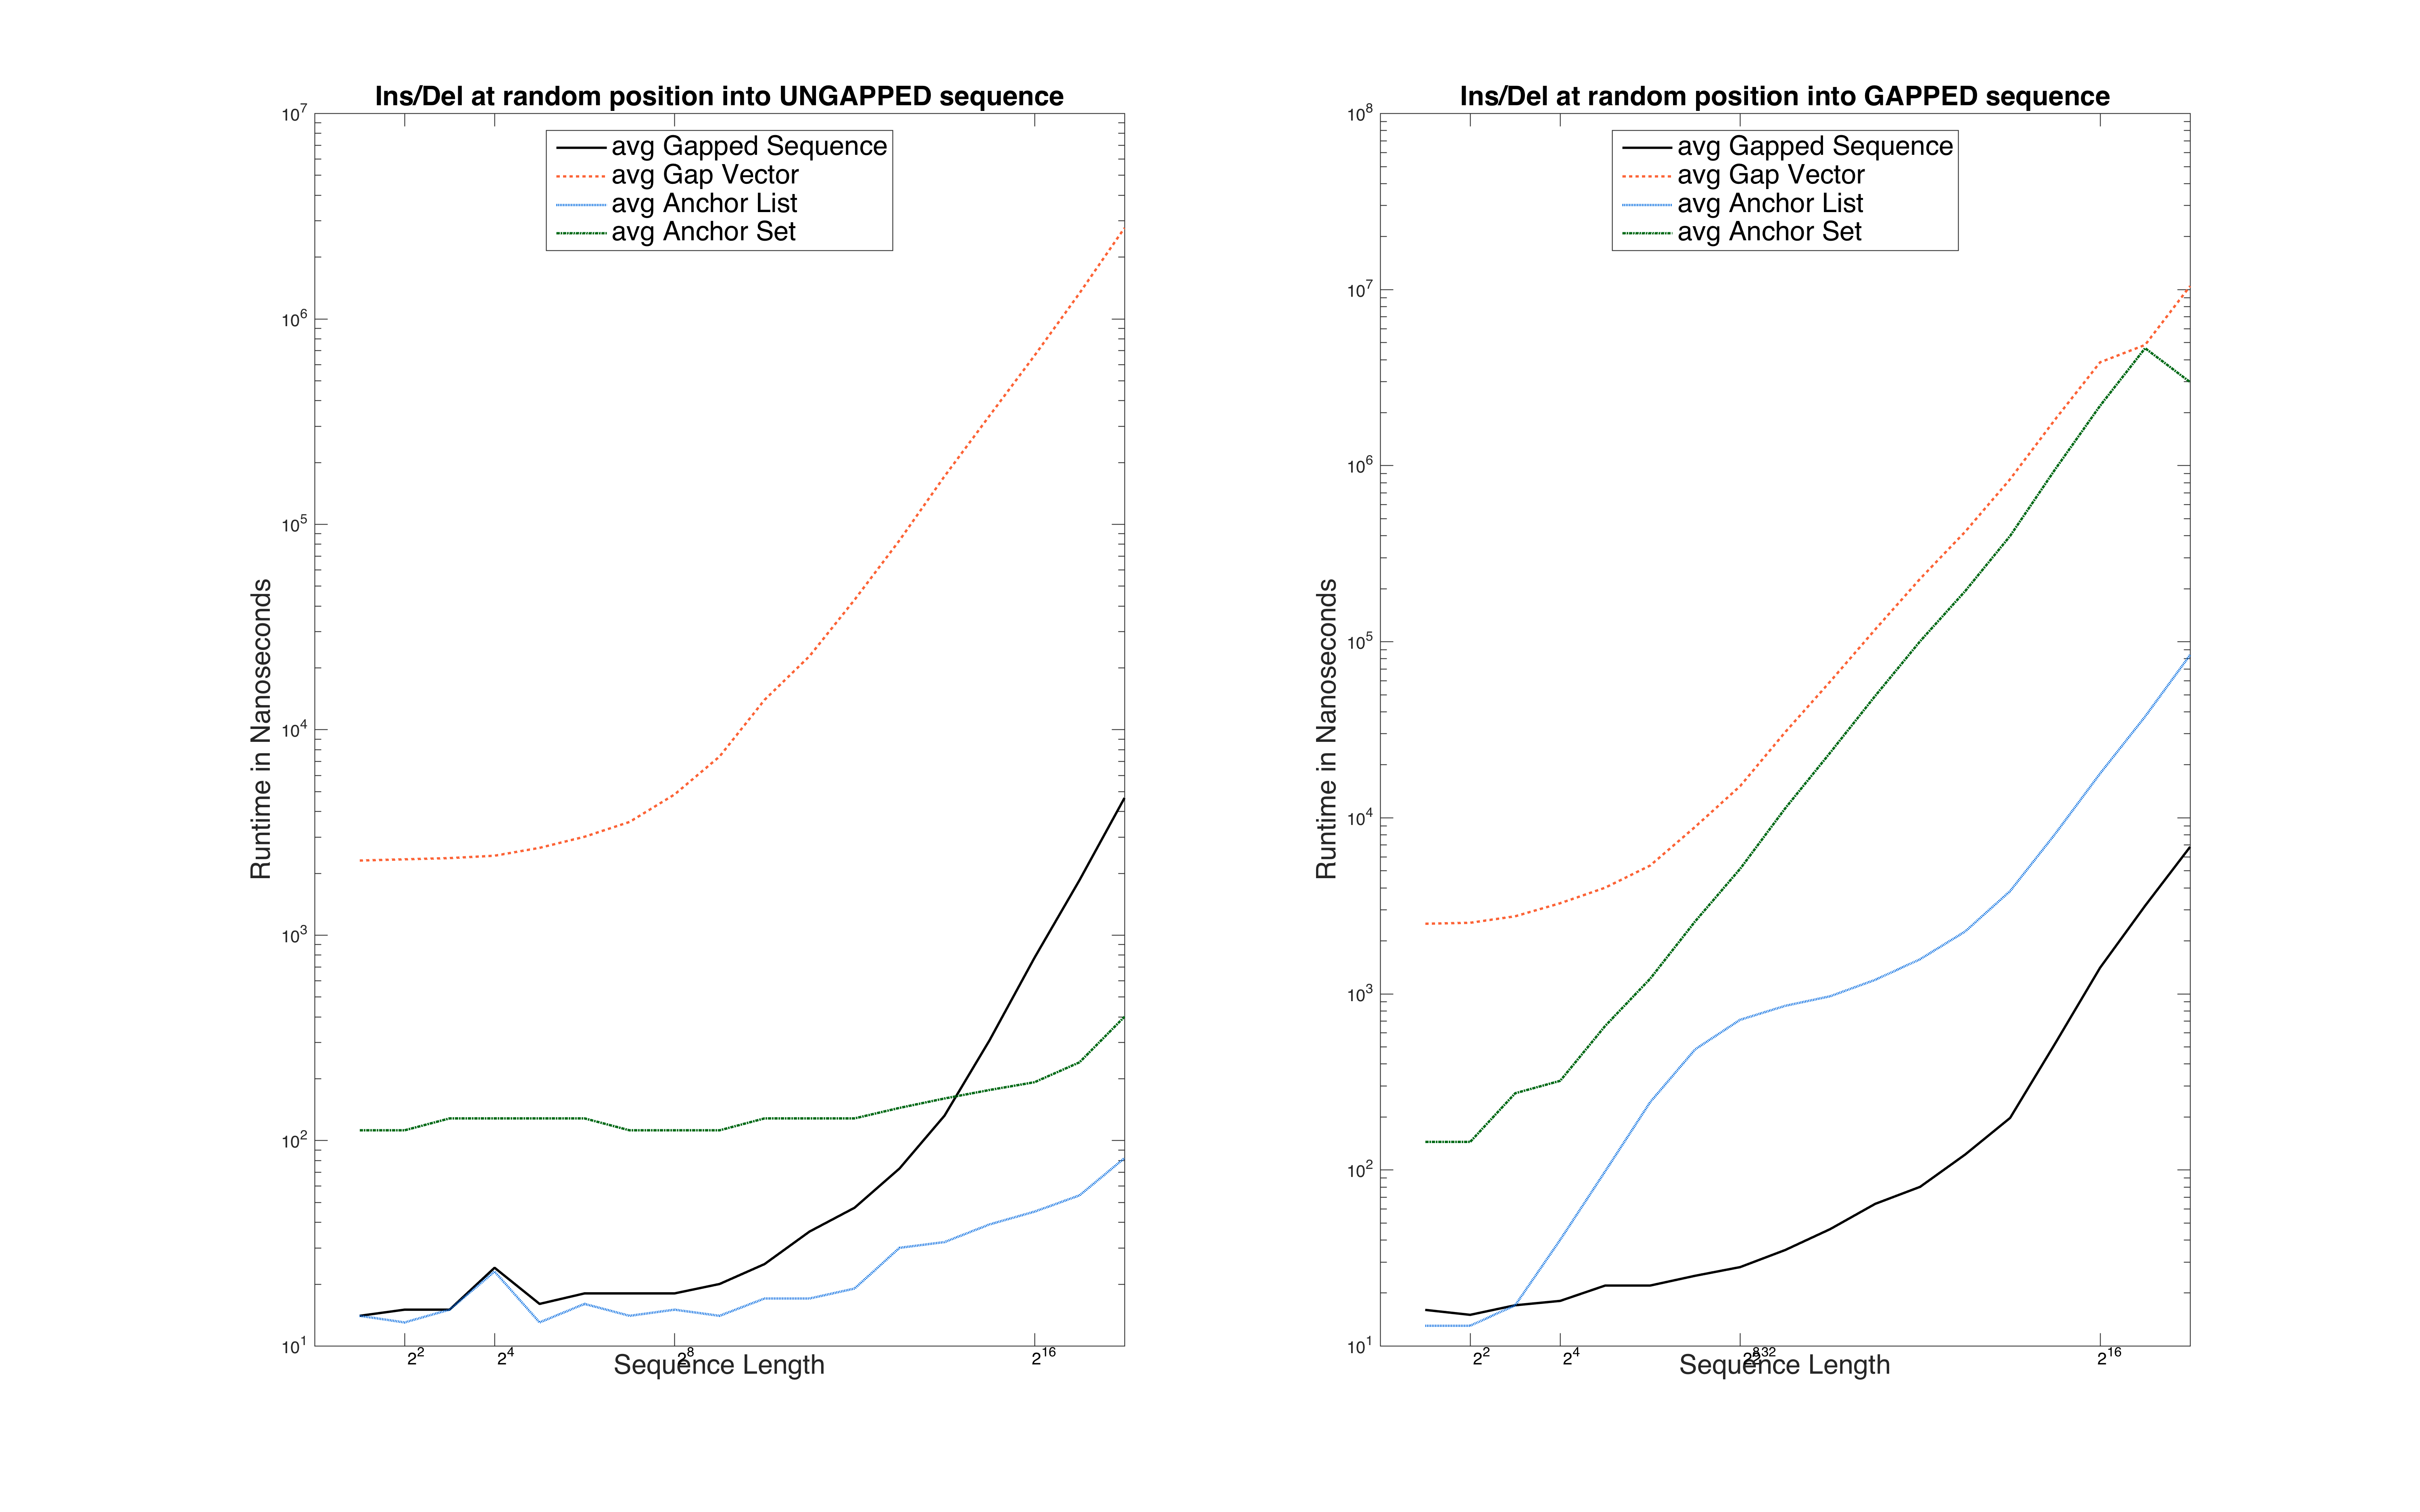
\includegraphics[scale=.4,trim={5cm 2cm 4.5cm 1.5cm},clip]{benchmark2_plot.png}
\caption{Left: Insert and delete at random positions into ungapped sequence. Right: 
Insert and delete at random positions into gapped sequence.}
\end{figure}

\begin{figure}[htpb]\centering
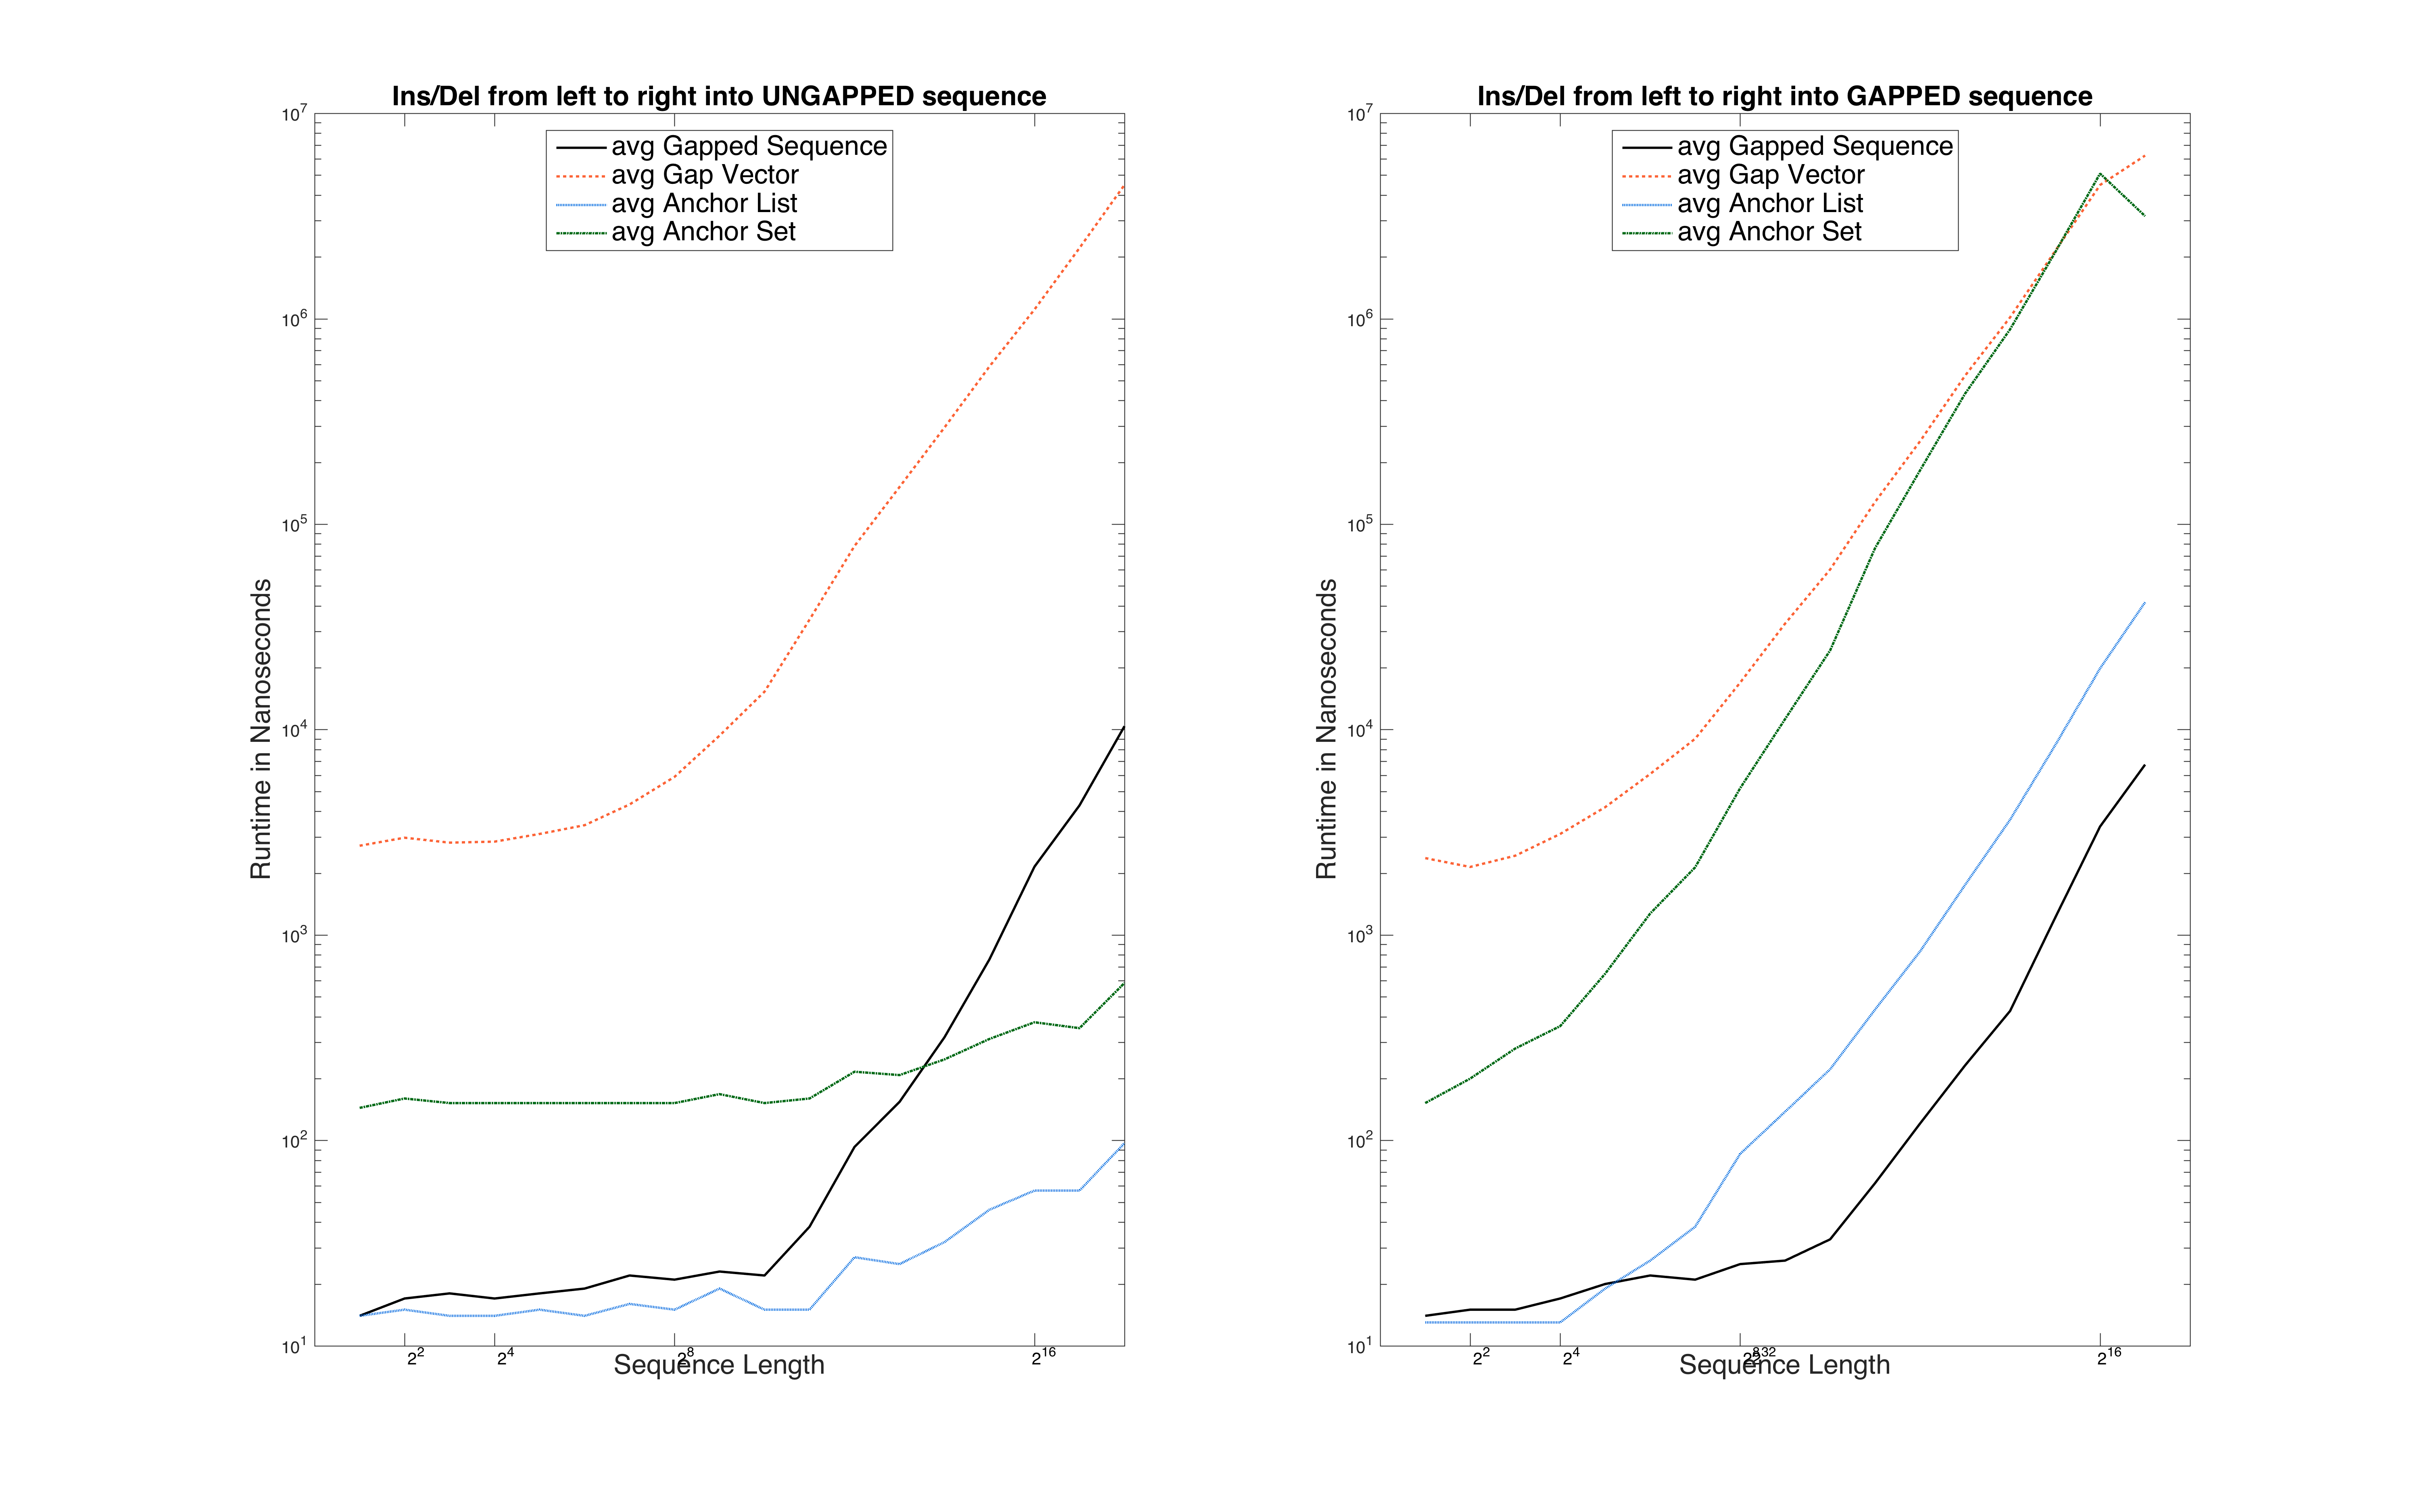
\includegraphics[scale=.4,trim={5cm 2cm 4.5cm 1.5cm},clip]{benchmark3_plot.png}
\caption{Left: Insert and delete from left to right into an ungapped sequence. Right: 
Insert and delete from left to right into a gapped sequence.}
\end{figure}

\section{Summary}
\subsection{Results}
\begin{itemize}
	\item The gapped sequence (\verb|gapped<dna15>|) always outperforms the other approaches, except when gaps are inserted from left to right into an empty sequence (see Benchmark 3). In this case the Anchor List approach is always faster, and the Anchor Set approach when sequence lengths exceeds $2^{12}$.
	\item The Gap Vector (\verb|sdsl::sd_vector|) never outperforms the three other approaches, but should be considered to be provided in SeqAn3 when only read operations are performed and a transformation to a \verb|gapped| sequence is undesirable. 
	\item When comparing anchor list versus anchor set for Benchmark 1 the anchor set outperforms the anchor list for sequence lengths exceeding $2^{12}$. However, both approaches are outperformed by the gap vector. For Benchmark 2 (insert/delete at random position) and Benchmark 3 (insert/delete from left to right) the anchor list always outperforms the anchor set.    
\end{itemize}

\subsection{Recommendations}
\begin{table}[htpb]\centering
\begin{tabular}{|l|l|l|}
\hline
\bf Usecase&\bf Data Structure\\
\hline
Read-Only&Gap Vector or Gapped Sequence\\
\hline
Ins/Del at Random Position into {\bf Ungapped} Sequence&Anchor List\\
\hline
Ins/Del at Random Position into {\bf Gapped} Sequence&Anchor List or Gapped Sequence\\
\hline
Ins/Del Left to Right into {\bf Ungapped} Sequence&Anchor List\\
\hline
Ins/Del Left to Right into {\bf Gapped} Sequence&Anchor List or Gapped Sequence\\
\hline
\end{tabular}
\end{table}

\end{document}
